\documentclass[11pt,fleqn,oneside]{book}

%%%%%%%%%%%%%%%%%%%%%%%%%%%%%%%%%%%%%%%%%
% Professional Book Structure
% LaTeX Template
%
% This file defines the structure and style of the book.
%%%%%%%%%%%%%%%%%%%%%%%%%%%%%%%%%%%%%%%%%

%----------------------------------------------------------------------------------------
%	PACKAGES AND OTHER DOCUMENT CONFIGURATIONS
%----------------------------------------------------------------------------------------

\usepackage[top=3cm,bottom=3cm,left=3cm,right=3cm,headsep=10pt,a4paper]{geometry} % Page margins

\usepackage[english]{babel} % English language
\usepackage[utf8]{inputenc} % Encoding
\usepackage[T1]{fontenc} % Font encoding
\usepackage{lmodern} % Modern font
%\usepackage{avant} % Use Avant Garde font for headings if desired

\usepackage{graphicx} % Images
\usepackage{enumitem} % Customized lists
\usepackage{booktabs} % Professional tables
\usepackage{xcolor} % Custom colors

%----------------------------------------------------------------------------------------
%	COLORS
%----------------------------------------------------------------------------------------

\definecolor{hfyellow}{RGB}{255, 204, 0} % Approx Hugging Face Yellow
\definecolor{hfdark}{RGB}{34, 34, 34}    % Dark Gray
\definecolor{hfblue}{RGB}{66, 133, 244}  % Blue accent
\definecolor{codebg}{RGB}{245, 245, 245} % Light gray for code blocks

%----------------------------------------------------------------------------------------
%	CODE SNIPPETS (LISTINGS)
%----------------------------------------------------------------------------------------

\usepackage{listings}
\lstset{
  basicstyle=\ttfamily\small,
  keywordstyle=\color{blue}\bfseries,
  commentstyle=\color{green!60!black},
  stringstyle=\color{red},
  backgroundcolor=\color{codebg},
  frame=single,
  rulecolor=\color{gray!30},
  breaklines=true,
  numbers=left,
  numberstyle=\tiny\color{gray},
  captionpos=b,
  tabsize=2,
  showstringspaces=false
}

%----------------------------------------------------------------------------------------
%	TIKZ & DIAGRAMS
%----------------------------------------------------------------------------------------

\usepackage{tikz}
\usetikzlibrary{shapes, arrows.meta, positioning, shadows, backgrounds, fit}

%----------------------------------------------------------------------------------------
%	CUSTOM BOXES (TCOLORBOX)
%----------------------------------------------------------------------------------------

\usepackage{tcolorbox}

% Definition Box
\newtcolorbox{infobox}[1][]{
  colback=blue!5!white,
  colframe=hfblue,
  fonttitle=\bfseries,
  title=Definition,
  boxrule=1pt,
  sharp corners=south,
  #1
}

% Concept/Explanation Box
\newtcolorbox{conceptbox}[1][]{
  colback=hfyellow!10!white,
  colframe=orange!80!black,
  fonttitle=\bfseries,
  title=Concept,
  boxrule=1pt,
  sharp corners=south,
  #1
}

% Warning/Note Box
\newtcolorbox{notebox}[1][]{
  colback=red!5!white,
  colframe=red!75!black,
  fonttitle=\bfseries,
  title=Note,
  boxrule=1pt,
  sharp corners=south,
  #1
}


%----------------------------------------------------------------------------------------
%	HEADERS AND FOOTERS
%----------------------------------------------------------------------------------------

\usepackage{fancyhdr}
\pagestyle{fancy}
\setlength{\headheight}{15pt} % Fix warning
\fancyhf{}
\fancyhead[L]{\nouppercase{\leftmark}} % Chapter name on the left
\fancyhead[R]{\thepage} % Page number on the right
\renewcommand{\headrulewidth}{0.5pt}

%----------------------------------------------------------------------------------------
%	TITLES
%----------------------------------------------------------------------------------------

\usepackage{titlesec}
\titleformat{\chapter}[display]
  {\normalfont\huge\bfseries\color{hfdark}}
  {\chaptertitlename\ \thechapter}
  {20pt}
  {\Huge}

%----------------------------------------------------------------------------------------
%	HYPERLINKS
%----------------------------------------------------------------------------------------

\usepackage{hyperref}
\hypersetup{
    colorlinks=true,
    linkcolor=hfblue,
    filecolor=magenta,      
    urlcolor=cyan,
    pdftitle={Hugging Face Book},
    pdfpagemode=FullScreen,
}
 % Load the structure.tex file

\begin{document}

%----------------------------------------------------------------------------------------
%	TITLE PAGE
%----------------------------------------------------------------------------------------

\begin{titlepage}
	\begin{tikzpicture}[remember picture, overlay]
		% Background color bar
		\fill[hfyellow] (current page.north west) rectangle ([xshift=4cm]current page.south west);
		
		% Decorative geometry
		\node[opacity=0.1, rotate=30] at ([xshift=8cm, yshift=-5cm]current page.north west) {
			\begin{tikzpicture}
				\node[draw, circle, minimum size=3cm, line width=2pt] (A) {};
				\node[draw, rectangle, minimum size=2cm, line width=2pt, below right=1cm of A] (B) {};
				\draw[line width=1pt] (A) -- (B);
			\end{tikzpicture}
		};

        % Title
		\node[anchor=north west, inner sep=0pt] at ([xshift=5cm, yshift=-8cm]current page.north west) {
			\begin{minipage}{0.7\paperwidth}
				\raggedright
				{\fontsize{40}{50}\selectfont \bfseries \color{hfdark} Hugging Face\\[10pt] \fontsize{30}{40}\selectfont \color{gray} The Comprehensive Guide}\\[1cm]
				{\Large \textit{From Transformers to Pipelines: A Visual Journey}}\\[2cm]
			\end{minipage}
		};

		% Author
		\node[anchor=south west, inner sep=0pt] at ([xshift=5cm, yshift=4cm]current page.south west) {
			\begin{minipage}{0.6\paperwidth}
				{\huge \bfseries Author: Mausam Kar}\\[0.5cm]
				{\large Written for Beginners \& Practitioners}
			\end{minipage}
		};
		
		% "Logo" or Visual Element
        \node[anchor=north east] at ([xshift=-2cm, yshift=-2cm]current page.north east) {
             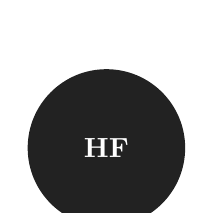
\begin{tikzpicture}
                \node[circle, fill=hfdark, minimum size=2cm, text=white, font=\bfseries] {HF};
             \end{tikzpicture}
        };

	\end{tikzpicture}
\end{titlepage}

%----------------------------------------------------------------------------------------
%	FRONT MATTER
%----------------------------------------------------------------------------------------

\tableofcontents

%----------------------------------------------------------------------------------------
%	MAIN CONTENT
%----------------------------------------------------------------------------------------

\mainmatter

\chapter{Getting Started with Hugging Face}

\section{What is Hugging Face?}
Hugging Face is often referred to as the \textbf{``GitHub of Machine Learning''}. It is an open-source platform that provides tools to build, train, and deploy machine learning models, primarily centered around \textit{Natural Language Processing (NLP)}.

At its core, Hugging Face democratizes AI by making state-of-the-art models accessible to everyone through the \texttt{transformers} library.

\begin{infobox}[title=Key Definition: Transformers]
    \textbf{Transformers} are a type of deep learning model designed to process sequential data, such as text. Introduced by Google in 2017 (in the paper \textit{"Attention is All You Need"}), they have revolutionized NLP by allowing models to understand context better than previous architectures like RNNs.
\end{infobox}

\section{The Pipeline Abstraction}
One of the easiest ways to use Hugging Face is through the \texttt{pipeline()} function. It abstracts away the complex code required to process text and generate predictions.

\begin{conceptbox}
    Think of a \textbf{Pipeline} as a factory assembly line. You pour raw material (text) into one end, and the finished product (sentiment, translation, summary) comes out the other end. The pipeline handles all the machinery inside.
\end{conceptbox}

\subsection{How it Works}
The pipeline consists of three main steps:
\begin{enumerate}
    \item \textbf{Preprocessing}: Converting text into numbers (Tokenization).
    \item \textbf{Inference}: Running the numbers through the Model.
    \item \textbf{Post-processing}: Converting the model's output back into human-readable text.
\end{enumerate}

\begin{center}
    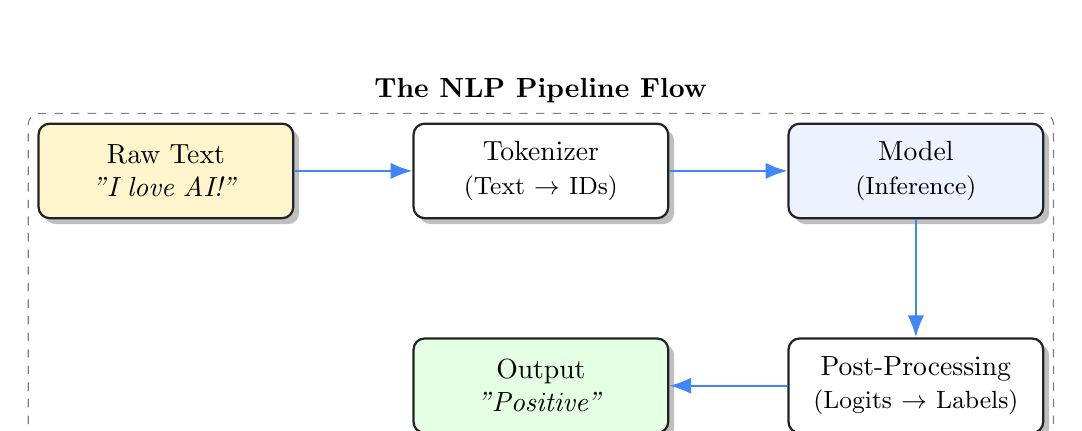
\begin{tikzpicture}[
        node distance=1.5cm,
        auto,
        block/.style={
            rectangle, 
            draw=hfdark, 
            thick, 
            fill=white, 
            text width=3cm, 
            align=center, 
            rounded corners, 
            minimum height=1.2cm, 
            drop shadow
        },
        arrow/.style={
            -{Latex[scale=1.2]}, 
            thick, 
            color=hfblue
        }
    ]
        % Nodes
        \node[block, fill=hfyellow!20] (input) {Raw Text\\ \textit{"I love AI!"}};
        \node[block, right=of input] (tokenizer) {Tokenizer\\ \small(Text $\to$ IDs)};
        \node[block, right=of tokenizer, fill=hfblue!10] (model) {Model\\ \small(Inference)};
        \node[block, below=of model] (post) {Post-Processing\\ \small(Logits $\to$ Labels)};
        \node[block, left=of post, fill=green!10] (output) {Output\\ \textit{"Positive"}};

        % Arrows
        \draw[arrow] (input) -- (tokenizer);
        \draw[arrow] (tokenizer) -- (model);
        \draw[arrow] (model) -- (post);
        \draw[arrow] (post) -- (output);
        
        % Background
        \begin{scope}[on background layer]
            \node[fit=(input)(tokenizer)(model)(post)(output), draw=gray, dashed, rounded corners, label=above:\textbf{The NLP Pipeline Flow}] {};
        \end{scope}
    \end{tikzpicture}
\end{center}

\section{Your First Code Example}
Let's see how simple it is to use Python to analyze the sentiment of a sentence.

\begin{lstlisting}[language=Python, caption=Basic Sentiment Analysis]
from transformers import pipeline

# 1. Initialize the pipeline
classifier = pipeline("sentiment-analysis")

# 2. Pass text to the pipeline
result = classifier("Hugging Face makes AI easy!")

# 3. Print the result
print(result)
# Output: [{'label': 'POSITIVE', 'score': 0.99}]
\end{lstlisting}

\begin{notebox}
    By default, the pipeline downloads a default model (like \texttt{distilbert}). You can specify other models if you need specific capabilities, such as multi-lingual support.
\end{notebox}

\section{Summary}
In this chapter, we learned:
\begin{itemize}
    \item \textbf{Hugging Face} is a platform for sharing and using ML models.
    \item \textbf{Pipelines} simplify the process of using these models.
    \item We can write a sentiment analysis script in just 3 lines of code!
\end{itemize}

\chapter{Models and Tokenizers}
\label{chap:models_tokenizers}

\section{Introduction}
While the \texttt{pipeline} API is powerful, it is often a "black box." To truly master Hugging Face, you must understand the two fundamental components that power every NLP application: \textbf{Tokenizers} and \textbf{Models}.

This chapter delves into the \texttt{AutoClasses}, the process of tokenization, and how to manage model configurations and weights.

\section{The AutoClasses}
Hugging Face provides a set of classes designed to automatically select the correct architecture for a given checkpoint. This design pattern makes your code incredibly flexible and portable.

\begin{infobox}[title=Key Classes]
    \begin{itemize}
        \item \texttt{AutoTokenizer}: Handles text preprocessing.
        \item \texttt{AutoModel}: Loads the base model (transformer body).
        \item \texttt{AutoConfig}: Manages technical parameters (layers, hidden size).
    \end{itemize}
\end{infobox}

\section{Tokenizers: Speaking the Language of Machines}
Deep Learning models cannot process raw strings. They require numerical input. The tokenizer bridges this gap by breaking text into smaller units called \textit{tokens} and mapping them to integers (\textit{Input IDs}).

\subsection{ The Tokenization Pipeline}
Tokenization isn't just splitting by spaces. It involves a sophisticated pipeline:

\begin{center}
    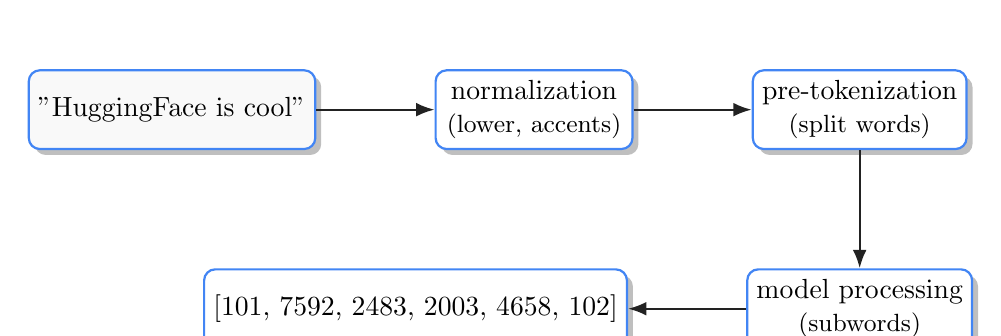
\begin{tikzpicture}[
        node distance=1.5cm, 
        auto,
        process/.style={
            rectangle, 
            draw=hfblue,
            thick,
            fill=white,
            minimum width=2.5cm,
            minimum height=1cm,
            align=center,
            rounded corners,
            drop shadow
        },
        arrow/.style={-{Latex}, thick, color=hfdark}
    ]
        \node[process, fill=gray!5] (raw) {"HuggingFace is cool"};
        \node[process, right=of raw] (norm) {normalization\\ \small(lower, accents)};
        \node[process, right=of norm] (pre) {pre-tokenization\\ \small(split words)};
        \node[process, below=of pre] (model) {model processing\\ \small(subwords)};
        \node[process, left=of model] (ids) {[101, 7592, 2483, 2003, 4658, 102]};
        
        \draw[arrow] (raw) -- (norm);
        \draw[arrow] (norm) -- (pre);
        \draw[arrow] (pre) -- (model);
        \draw[arrow] (model) -- (ids);
        
    \end{tikzpicture}
\end{center}

\begin{conceptbox}
    \textbf{Subword Tokenization}: Algorithms like BPE (Byte-Pair Encoding) or WordPiece solve the "unknown token" problem. They split rare words into common subwords.
    
    Example: \texttt{"unfriendly"} $\rightarrow$ \texttt{"un", "friend", "ly"}
\end{conceptbox}

\section{Using AutoTokenizer}
Here is a complete example of loading a tokenizer and processing a batch of sentences.

\begin{lstlisting}[language=Python, caption=Processing a Batch]
from transformers import AutoTokenizer

# 1. Load a pre-trained tokenizer
checkpoint = "bert-base-cased"
tokenizer = AutoTokenizer.from_pretrained(checkpoint)

# 2. Define a batch of sentences
batch = [
    "Hello, world!",
    "Hugging Face course is amazing."
]

# 3. Tokenize
# padding: pad short sequences to the longest in batch
# truncation: cut sequences longer than model max length
inputs = tokenizer(
    batch, 
    padding=True, 
    truncation=True, 
    return_tensors="pt" # Return PyTorch tensors
)

print(inputs)
# Outputs dictionary with 'input_ids', 'attention_mask'
\end{lstlisting}

\section{Models and Configurations}
The \texttt{AutoModel} class loads the weights of the network. However, sometimes you want to inspect or modify the architecture before loading the weights. This is where \texttt{AutoConfig} comes in.

\begin{lstlisting}[language=Python, caption=Customizing Configuration]
from transformers import AutoConfig, AutoModel

# Load the default configuration
config = AutoConfig.from_pretrained("bert-base-uncased")

# Inspect a parameter
print(config.hidden_size) # 768

# Modify it (e.g., for a smaller custom model)
config.num_hidden_layers = 10

# Initialize a model with this config (Random weights!)
model = AutoModel.from_config(config)
\end{lstlisting}

\begin{notebox}
    Initializing from config loads \textbf{random weights}. You must use \texttt{from\_pretrained()} to load trained knowledge.
\end{notebox}

\section{Saving Your Work}
After fine-tuning or modifying a model, you need to save it. Hugging Face makes this easy with \texttt{save\_pretrained}.

\begin{lstlisting}[language=Python]
# Save tokenizer and model to a local directory
save_directory = "./my_saved_model"

tokenizer.save_pretrained(save_directory)
model.save_pretrained(save_directory)

# You can now load from this directory!
loaded_model = AutoModel.from_pretrained(save_directory)
\end{lstlisting}

\section{Summary}
In this chapter, we explored:
\begin{itemize}
    \item How \textbf{Tokenizers} transform text into input IDs using algorithms like BPE.
    \item The role of \textbf{AutoConfig} in defining model architecture.
    \item How to \textbf{Save and Load} models locally, ensuring your work is never lost.
\end{itemize}

\chapter{The Datasets Library}
\label{chap:datasets}

\section{Introduction}
Good models perform poorly on bad data. The Hugging Face \texttt{datasets} library is the standard tool for loading, processing, and sharing datasets in the NLP ecosystem. It is designed to be efficient, developer-friendly, and compatible with NumPy, Pandas, and PyTorch/TensorFlow.

\section{Loading Data}
Hugging Face hosts thousands of datasets on the Hub, but you will often work with your own local files.

\subsection{From the Hub}
\begin{lstlisting}[language=Python]
from datasets import load_dataset

# Load a benchmark dataset (GLUE)
glue_dataset = load_dataset("glue", "mrpc", split="train")
\end{lstlisting}

\subsection{From Local Files}
The library supports loading directly from CSV, JSON, and text files.

\begin{lstlisting}[language=Python, caption=Loading Local Files]
# Load from a single CSV
data_files = {"train": "path/to/train.csv", "test": "path/to/test.csv"}
dataset = load_dataset("csv", data_files=data_files)

# Load from JSON Lines
json_dataset = load_dataset("json", data_files="my_data.jsonl")
\end{lstlisting}

\section{Inspecting Data with Pandas}
Sometimes you just want to "see" your data. The \texttt{datasets} library integrates seamlessly with Pandas.

\begin{lstlisting}[language=Python, caption=Converting to Pandas DataFrame]
import pandas as pd

# Convert to pandas
df = glue_dataset.to_pandas()

# Show the first 5 rows
print(df.head())
\end{lstlisting}

\begin{infobox}[title=Efficiency Note]
    The conversion to Pandas is purely in-memory. For massive datasets, you should avoid this or converting only a small slice.
\end{infobox}

\section{Processing Data: Slicing and Mapping}
\subsection{Slicing and Shuffling}
You can manipulate datasets just like python lists context.

\begin{lstlisting}[language=Python]
# Shuffle the dataset
shuffled = dataset.shuffle(seed=42)

# Select the first 1000 examples
small_dataset = dataset.select(range(1000))
\end{lstlisting}

\subsection{The Map Function}
The core powerhouse of the library is \texttt{.map()}. It allows you to apply processing functions (like tokenization) to every element.

\begin{conceptbox}
    \textbf{Why \texttt{batched=True}?}
    
    Tokenizers are written in Rust and can process lists of texts much faster than single strings thanks to parallelism. Enabling batching can speed up your processing by 10x or 100x.
\end{conceptbox}

\begin{lstlisting}[language=Python, caption=High-Performance Tokenization]
def tokenize_function(examples):
    # 'examples["text"]' is a LIST of strings
    return tokenizer(examples["text"], truncation=True)

# Apply to the whole dataset
tokenized_dataset = dataset.map(tokenize_function, batched=True)
\end{lstlisting}

\section{Streaming: Handling Big Data}
What if your dataset is 1TB and your laptop has 16GB of RAM? Enter \textbf{Streaming}.

Streaming allows you to iterate over a dataset without downloading it to disk. It streams data over the network on-the-fly.

\begin{lstlisting}[language=Python]
# This returns an IterableDataset
c4 = load_dataset("c4", "en", streaming=True)

# Get the first example
print(next(iter(c4)))
\end{lstlisting}

\section{Summary}
We have covered:
\begin{itemize}
    \item Loading data from the Hub and local CSV/JSON files.
    \item Interoperating with Pandas for visualization.
    \item Using \texttt{map()} for efficient preprocessing.
    \item Handling massive datasets with Streaming.
\end{itemize}

\chapter{Fine-Tuning Your First Model}
\label{chap:finetuning}

\section{The Concept of Transfer Learning}
Traditional machine learning required training models from scratch on specific datasets. In the era of large language models, this is inefficient.

\textbf{Transfer Learning} allows us to take a model trained on a massive generic corpus (like Wikipedia) and "fine-tune" it on a small, task-specific dataset (like your company's emails).

\begin{infobox}[title=The Head Analogy]
    Imagine the model as a body and a head.
    \begin{itemize}
        \item \textbf{Body}: Contains general language understanding (grammar, context). This is Frozen or fine-tuned slightly.
        \item \textbf{Head}: The final layer responsible for the output (e.g., "Positive/Negative"). This is \textbf{randomly initialized} and trained from scratch.
    \end{itemize}
\end{infobox}

\section{The Trainer API}
The \texttt{Trainer} class is a high-level API that abstracts away the complex training loop of PyTorch (optimizers, backward pass, gradient accumulation).

\subsection{1. Computing Metrics}
By default, the Trainer only logs the loss. To know if your model is actually working (Accuracy, F1), we need a \texttt{compute\_metrics} function.

\begin{lstlisting}[language=Python]
import numpy as np
import evaluate

metric = evaluate.load("accuracy")

def compute_metrics(eval_pred):
    logits, labels = eval_pred
    predictions = np.argmax(logits, axis=-1)
    return metric.compute(predictions=predictions, references=labels)
\end{lstlisting}

\subsection{2. Training Arguments}
These control "how" the model learns.

\begin{lstlisting}[language=Python, caption=Essential Hyperparameters]
from transformers import TrainingArguments

args = TrainingArguments(
    output_dir="./results",
    # Evaluation strategy: evaluate every epoch
    evaluation_strategy="epoch", 
    # Learning rate: usually very small for Transfer Learning
    learning_rate=2e-5,
    per_device_train_batch_size=16,
    num_train_epochs=3,
    # Weight decay: regularization technique
    weight_decay=0.01,
)
\end{lstlisting}

\subsection{3. Launching Training}
Combine the model, args, data, and metrics into the Trainer.

\begin{lstlisting}[language=Python]
from transformers import Trainer

trainer = Trainer(
    model=model,
    args=args,
    train_dataset=tokenized_datasets["train"],
    eval_dataset=tokenized_datasets["test"],
    tokenizer=tokenizer,
    compute_metrics=compute_metrics,
)

trainer.train()
\end{lstlisting}

\section{Checkpoints and Resuming}
Training can take hours. What if your computer crashes? The Trainer defines \texttt{save\_steps} to save checkpoints automatically.

To resume training from the latest checkpoint:
\begin{lstlisting}[language=Python]
trainer.train(resume_from_checkpoint=True)
\end{lstlisting}

\section{Summary}
Fine-tuning adapts a powerful general model to your specific needs. The \texttt{Trainer} API simplifies the training loop, evaluation, and checkpoint management, letting you focus on the data and the results.

\chapter{The Hugging Face Hub}
\label{chap:hub}

\section{The GitHub of Machine Learning}
The Hugging Face Hub constitutes the central repository of the NLP community. It hosts over 300,000 models, 50,000 datasets, and thousands of demo applications (Spaces).

\section{Authentication: The CLI}
To interact with the Hub (uploading models), you need to authenticate. The command-line interface (CLI) is the easiest way to do this.

\begin{lstlisting}[language=bash, caption=Login via Terminal]
$ huggingface-cli login

# You will be asked to enter your token from:
# https://huggingface.co/settings/tokens
\end{lstlisting}

\begin{infobox}[title=Git Integration]
    Under the hood, every model on the Hub is a Git repository. You can \texttt{git clone}, \texttt{git add}, and \texttt{git push} large model files (using Git LFS) just like you would with code.
\end{infobox}

\section{Model Cards: Documentation Matters}
A model without documentation is useless. The "Model Card" is the \texttt{README.md} file of your repository. It contains:
\begin{itemize}
    \item \textbf{Model Description}: What does it do?
    \item \textbf{Intended Use}: What are the valid use cases?
    \item \textbf{Limitations}: Bias and risks.
    \item \textbf{Training Data}: What data was it trained on?
\end{itemize}

\subsection{Metadata tags}
Model cards start with a YAML header that helps the Hub filter your model.
\begin{verbatim}
---
language: en
tags:
- text-classification
- pytorch
datasets:
- glue
metrics:
- accuracy
---
\end{verbatim}

\section{Hugging Face Spaces}
Spaces are slightly different from Model repos. They are designed to host \textit{running applications}.

\subsection{SDKs: Gradio vs Streamlit}
\begin{itemize}
    \item \textbf{Gradio}: Built by Hugging Face. Extremely simple, "Python-function-to-UI" approach. Best for quick demos.
    \item \textbf{Streamlit}: More flexible, dashboard-oriented. Great for data exploration apps.
\end{itemize}

\begin{lstlisting}[language=Python, caption=A Full Gradio App]
import gradio as gr
from transformers import pipeline

classifier = pipeline("sentiment-analysis")

def predict(text):
    return classifier(text)[0]

# Launch the interface
gr.Interface(
    fn=predict, 
    inputs="text", 
    outputs="label",
    title="My Sentiment Analyzer"
).launch()
\end{lstlisting}

\section{Conclusion}
You have now journeyed from the basics of tokenization to training your own models and sharing them with the world. The Hugging Face ecosystem is vast, but you have the keys to explore it.

\begin{center}
    \textit{"The magic of AI is not in the models, but in what you build with them."}
\end{center}


% Future chapters can be included here
% \chapter{Models and Tokenizers}
\label{chap:models_tokenizers}

\section{Introduction}
While the \texttt{pipeline} API is powerful, it is often a "black box." To truly master Hugging Face, you must understand the two fundamental components that power every NLP application: \textbf{Tokenizers} and \textbf{Models}.

This chapter delves into the \texttt{AutoClasses}, the process of tokenization, and how to manage model configurations and weights.

\section{The AutoClasses}
Hugging Face provides a set of classes designed to automatically select the correct architecture for a given checkpoint. This design pattern makes your code incredibly flexible and portable.

\begin{infobox}[title=Key Classes]
    \begin{itemize}
        \item \texttt{AutoTokenizer}: Handles text preprocessing.
        \item \texttt{AutoModel}: Loads the base model (transformer body).
        \item \texttt{AutoConfig}: Manages technical parameters (layers, hidden size).
    \end{itemize}
\end{infobox}

\section{Tokenizers: Speaking the Language of Machines}
Deep Learning models cannot process raw strings. They require numerical input. The tokenizer bridges this gap by breaking text into smaller units called \textit{tokens} and mapping them to integers (\textit{Input IDs}).

\subsection{ The Tokenization Pipeline}
Tokenization isn't just splitting by spaces. It involves a sophisticated pipeline:

\begin{center}
    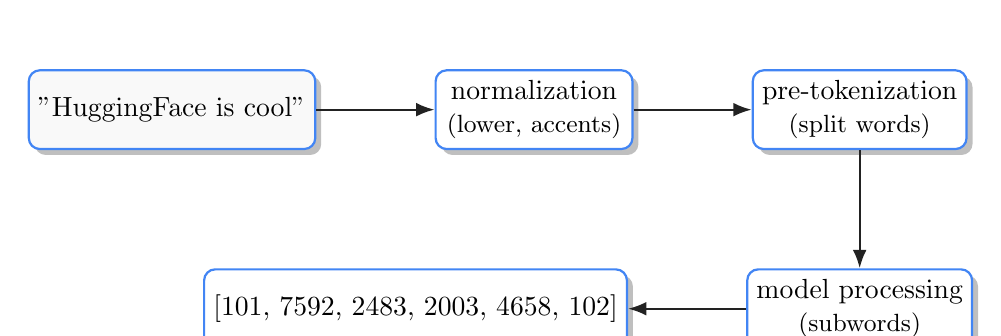
\begin{tikzpicture}[
        node distance=1.5cm, 
        auto,
        process/.style={
            rectangle, 
            draw=hfblue,
            thick,
            fill=white,
            minimum width=2.5cm,
            minimum height=1cm,
            align=center,
            rounded corners,
            drop shadow
        },
        arrow/.style={-{Latex}, thick, color=hfdark}
    ]
        \node[process, fill=gray!5] (raw) {"HuggingFace is cool"};
        \node[process, right=of raw] (norm) {normalization\\ \small(lower, accents)};
        \node[process, right=of norm] (pre) {pre-tokenization\\ \small(split words)};
        \node[process, below=of pre] (model) {model processing\\ \small(subwords)};
        \node[process, left=of model] (ids) {[101, 7592, 2483, 2003, 4658, 102]};
        
        \draw[arrow] (raw) -- (norm);
        \draw[arrow] (norm) -- (pre);
        \draw[arrow] (pre) -- (model);
        \draw[arrow] (model) -- (ids);
        
    \end{tikzpicture}
\end{center}

\begin{conceptbox}
    \textbf{Subword Tokenization}: Algorithms like BPE (Byte-Pair Encoding) or WordPiece solve the "unknown token" problem. They split rare words into common subwords.
    
    Example: \texttt{"unfriendly"} $\rightarrow$ \texttt{"un", "friend", "ly"}
\end{conceptbox}

\section{Using AutoTokenizer}
Here is a complete example of loading a tokenizer and processing a batch of sentences.

\begin{lstlisting}[language=Python, caption=Processing a Batch]
from transformers import AutoTokenizer

# 1. Load a pre-trained tokenizer
checkpoint = "bert-base-cased"
tokenizer = AutoTokenizer.from_pretrained(checkpoint)

# 2. Define a batch of sentences
batch = [
    "Hello, world!",
    "Hugging Face course is amazing."
]

# 3. Tokenize
# padding: pad short sequences to the longest in batch
# truncation: cut sequences longer than model max length
inputs = tokenizer(
    batch, 
    padding=True, 
    truncation=True, 
    return_tensors="pt" # Return PyTorch tensors
)

print(inputs)
# Outputs dictionary with 'input_ids', 'attention_mask'
\end{lstlisting}

\section{Models and Configurations}
The \texttt{AutoModel} class loads the weights of the network. However, sometimes you want to inspect or modify the architecture before loading the weights. This is where \texttt{AutoConfig} comes in.

\begin{lstlisting}[language=Python, caption=Customizing Configuration]
from transformers import AutoConfig, AutoModel

# Load the default configuration
config = AutoConfig.from_pretrained("bert-base-uncased")

# Inspect a parameter
print(config.hidden_size) # 768

# Modify it (e.g., for a smaller custom model)
config.num_hidden_layers = 10

# Initialize a model with this config (Random weights!)
model = AutoModel.from_config(config)
\end{lstlisting}

\begin{notebox}
    Initializing from config loads \textbf{random weights}. You must use \texttt{from\_pretrained()} to load trained knowledge.
\end{notebox}

\section{Saving Your Work}
After fine-tuning or modifying a model, you need to save it. Hugging Face makes this easy with \texttt{save\_pretrained}.

\begin{lstlisting}[language=Python]
# Save tokenizer and model to a local directory
save_directory = "./my_saved_model"

tokenizer.save_pretrained(save_directory)
model.save_pretrained(save_directory)

# You can now load from this directory!
loaded_model = AutoModel.from_pretrained(save_directory)
\end{lstlisting}

\section{Summary}
In this chapter, we explored:
\begin{itemize}
    \item How \textbf{Tokenizers} transform text into input IDs using algorithms like BPE.
    \item The role of \textbf{AutoConfig} in defining model architecture.
    \item How to \textbf{Save and Load} models locally, ensuring your work is never lost.
\end{itemize}


\end{document}
